\documentclass{article}
\usepackage[margin=1.0in]{geometry}

\usepackage{amsmath}
\usepackage{amsfonts}
\usepackage{amssymb}
\usepackage{graphicx}
\usepackage[hidelinks]{hyperref}
\usepackage{lineno}
\usepackage{booktabs}

\usepackage{graphicx}
\usepackage{caption}
\usepackage{subcaption}
\usepackage{hyperref}

\usepackage{listings}
\usepackage{xcolor}

\colorlet{punct}{red!60!black}
\definecolor{background}{HTML}{EEEEEE}
\definecolor{delim}{RGB}{20,105,176}
\colorlet{numb}{magenta!60!black}

\lstdefinelanguage{json}{
    basicstyle=\normalfont\ttfamily,
    numbersep=8pt,
    showstringspaces=false,
    breaklines=true,
    literate=
     *{0}{{{\color{numb}0}}}{1}
      {1}{{{\color{numb}1}}}{1}
      {2}{{{\color{numb}2}}}{1}
      {3}{{{\color{numb}3}}}{1}
      {4}{{{\color{numb}4}}}{1}
      {5}{{{\color{numb}5}}}{1}
      {6}{{{\color{numb}6}}}{1}
      {7}{{{\color{numb}7}}}{1}
      {8}{{{\color{numb}8}}}{1}
      {9}{{{\color{numb}9}}}{1}
      {:}{{{\color{punct}{:}}}}{1}
      {,}{{{\color{punct}{,}}}}{1}
      {\{}{{{\color{delim}{\{}}}}{1}
      {\}}{{{\color{delim}{\}}}}}{1}
      %{[}{{{\color{delim}{[}}}}{1}
      %{]}{{{\color{delim}{]}}}}{1},
}

\linenumbers

\newcommand{\median}{\operatorname{median}}

% http://bytesizebio.net/2013/03/11/adding-supplementary-tables-and-figures-in-latex/
\newcommand{\beginsupplement}{%
        \setcounter{table}{0}
        \renewcommand{\thetable}{S\arabic{table}}%
        \setcounter{figure}{0}
        \renewcommand{\thefigure}{S\arabic{figure}}%
     }

\hyphenation{Ge-nome Ge-nomes hyper-mut-ation through-put}

\title{Methods used for PhIP-Seq Data Analysis}
\author{Caitlin et. al}

\begin{document}
\maketitle

%\begin{abstract}
%\end{abstract}

\paragraph{Alignment Pipeline}

The enrichment matrix was created by aligning all samples to the reference library using a \textbf{Nextflow} data processing pipeline.
The pipeline starts with the metadata for all samples (including a path to the fastq reads) 
as well as the metadata for all the peptides in the library.
The processing steps are as follows:
(1) Build a \textbf{Bowtie} CITE\cite{} index from the peptide metadata by converting the metadata to fasta format and feeding into the \textbf{bowtie-build} command.
(2) Align each of the samples to the library using \textbf{Bowtie} end-to-end alignment allowing for up to 2 mismatches. 
Each of the reads is $125$bp long, so we trim the low quality end of the read to match the reference length, $117$bp, before alignment.
(3) The pipeline extracts the counts of each peptide in each sample alignment by using \textbf{samtools-idxstats} CITE\cite{}.
(4) Finally, all the individual counts information for each sample are merged into a single raw counts \textit{enrichment} matrix.
The final result of the alignment pipeline is a dataset containing the enrichment matrix, sample metadata, and peptide metadata organized into a coherent 
dataset using the \textbf{xarray} CITE\cite{} package.

\paragraph{Sample curation and model fit groups}

Each sample in our dataset is defined by a single Immuno-Precipitation (IP) experiment with a serum antibody sample and library batch of phage-displayed peptides.
To be sure our results are reproducible, we curate results from samples using two classes of replicates for each serum sample. 
\textit{technical replicates} represent a set of samples which are from the same serum sample. 
The IP experiments for each technical replicate use the same library batch, and are performed by the same person on the same day.
\textit{biological replicates} are defined by IP experiments done on a different day with a split serum draw; may be the same or different libraries.
The first step of sample curation is a $0.5$ threshold of correlation between the counts of all technical replicates.
The counts of the samples above this threshold are then averaged to make a single reproducible biological replicate.
For data from a serum to be included in the final analysis, it must have a reproducible biological replicate using both library batches.
Then for each sample, we take the two biological replicates with highest technical replicate reproducibility, 
such that the two were not generated using the same library 
After sample curation we are left with two sample sets divided by the library batch used for respective sample IP experiments.
% each with respect to the phage library batch used during the IP experiment.
Concretely, each serum sample's results in the analysis is represented by a biological replicate IP using each of the two library batches.

\paragraph{Assessing significance using a Gamma-Poisson model}

We observe noise introduced by library peptide abundance and ``sticky" peptide bias.
To parse this, each of the two curated sample sets are fit to a Gamma-Poisson mixture model first introduced by \textbf{phip-stat} CITE\cite{}.
We fit each model with a number of mock-IP controls to give us information 
about abundance and false binding affinity for each peptide in the library.
To control for the variance in sequencing coverage between samples, we first normalize all samples
using counts factor method as seen in CITE\cite{}.
This leaves us with a normalized raw counts matrix, $M_{i,j}$, for $i$ peptides and $j$ samples.
The model assumes that each entry in the count matrix, for any given peptide $i$, is sampled from a Poisson distribution with rate, $\lambda_{i}$.
Next, we assume the prior distribution for each possible $\lambda_{i}$ is pulled from a Gamma distribution 
defined by $\alpha$ and $\beta$ (inverse scale) parameters.
We then infer these parameters by looking at the set of mean normalize counts for each peptide
using the \textbf{scipy.optimize} CITE\cite{} package.
Given the posterior of the rate is also Gamma distributed, the posterior hyperparameters are thus defined
$\alpha^{'} = \alpha + \sum_{i}^{n}x_{i}$, $\beta^{'} = \beta + n$.
Given these, $\lambda_{i} = \alpha^{'}_{i}/\beta^{'}_{i}$.
Finally, we get $-log10(pval)$ (MLXP) values by computing the size of the tail of the Poisson distribution for each normalized sample count at peptide, $i$.

%\paragraph{Control peptide ratio for false positive rate}

%\paragraph{Hit calling}

%\section*{}

%\begin{figure}
%\centering
%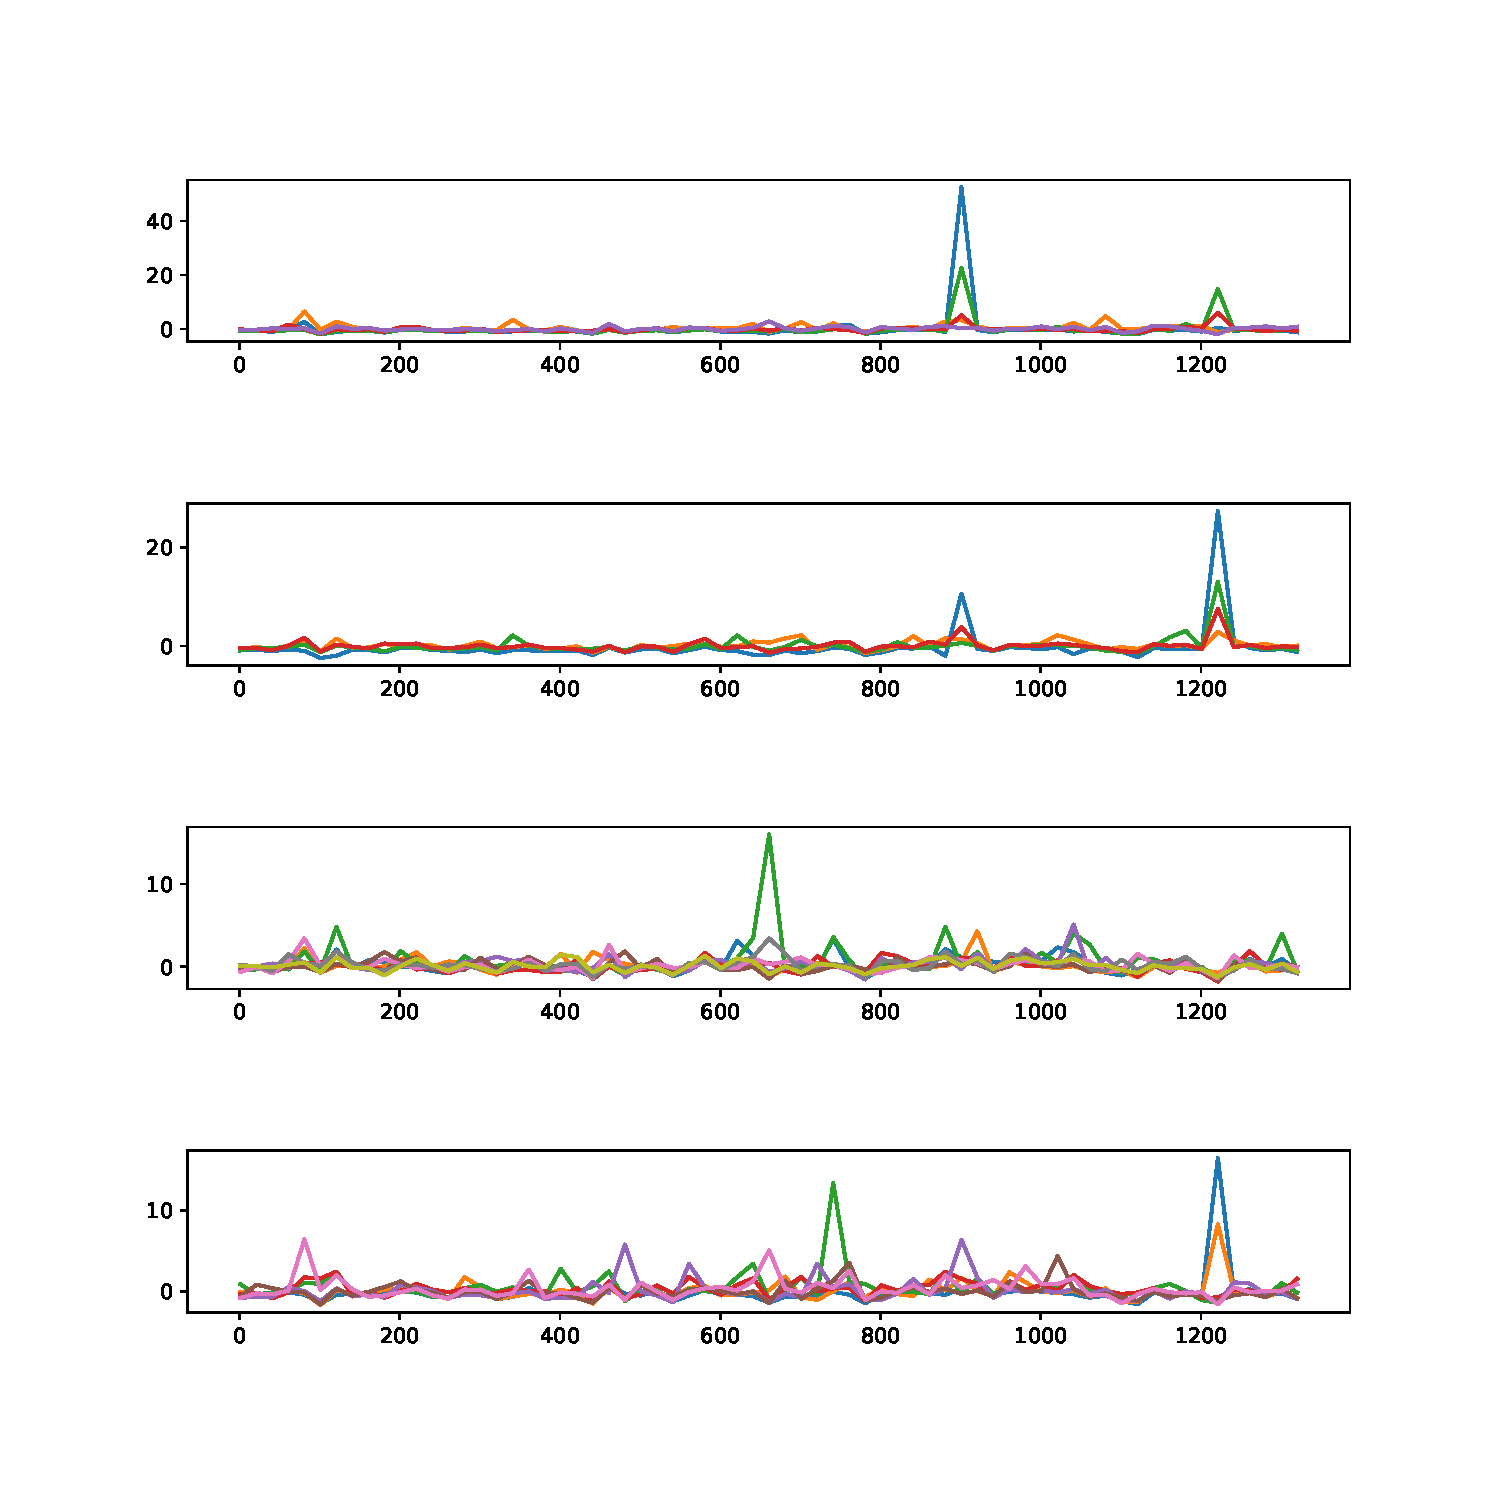
\includegraphics[width=1.0\textwidth]{figures/ANON_split.pdf}
%\caption{ \
%Standardized enrichment for strain <X>, plotted as a function of tile genomic location. The samples are then grouped by a column in the sample metadata column.
%}
%\label{fig:anon_split}
%\end{figure}

%\clearpage
%\bibliographystyle{plain}
%\bibliography{main}

% \clearpage
% \section*{Supplementary Materials}
% \beginsupplement
% Supplementary text and figures here.

\end{document}




